\section{Results}
\label{section:results}

% Intro
% TEST 1: simulations
%-----------------------------------------------------------------------------
%   - The simulated data
%   - The results
% PLOT: histograms over inferred ages (1) just isochrones (2) just
% gyrochronology, (3) both.

% TEST 2: Clusters
%-----------------------------------------------------------------------------
%   - The cluster data
%   - The results
% PLOT: histograms over inferred ages (1) just isochrones (2) just
% gyrochronology, (3) both.

% Rolling out/future
%   - Adding new datasets/dimensions/methods.
%-----------------------------------------------------------------------------

% Intro
%-----------------------------------------------------------------------------
In order to demonstrate the functionality of our method, we conducted two
tests.
In the first we simulated a set of observables from a set of fundamental
parameters for a few hundred stars using the MIST \citep{choi} stellar
evolution models.
In the second we tested our model by attempting the measure the ages of stars
in the Praesepe open cluster who's age has been measured precisely because it
is an ensemble of coeval stars with the same metallicity; a single stellar
poplulation, and its age can be established through isochrone fitting and MS
turn-off.

% TEST 1: simulations
%-----------------------------------------------------------------------------
%   - The simulated data
For the first test we began with a set of 1000 stars and drew masses, ages,
bulk metallicities, distances and extinctions at random from the following
uniform distributions:
\begin{eqnarray}
& M \sim U(0.5, 1.5)~[M_\odot] \\
& A \sim U(0.5, 14)\mathrm{~[Gyr]} \\
& F \sim U(-0.2, 0.2) \\
& D \sim U(10, 1000)~\mathrm{[pc]} \\
& A_V \sim U(0, 1).
\end{eqnarray}
\teff, \logg, \fhat, {\bf \mx}, \pmega\ and B-V were then generated using
these stellar parameters with the MIST stellar evolution models \citep{choi}
and rotation periods, $P$ were generated from the gyrochronology relation in
equation \ref{eqn:gyro} with age, $A$, and B-V.
% Uncertainties.
We then performed cuts on these simulated stars to remove evolved stars and
stars that are too hot.
The rotation periods of evolved stars, defined here to be those with \logg\ >
4.5 begin to increase as soon as they turn off the MS and their radii start to
enlarge and cannot be modeled with the gyrochronology relation of equation
\ref{eqn:gyro_age}.
In addition, hot stars (defined as 6250 K < \teff) cannot be modeled using
equation \ref{eqn:gyro_age} because their convective envelopes are extremely
shallow and their magnetic fields are weaker, leading to a lack of magnetic
braking.
The rotation periods of these stars do not increase substantially during their
time on the MS.
After performing these cuts, 649 \racomment{update} stars remained in the
sample of simulated stars.
% We attempted to measure the ages of the stars in this sample using the method
% outlined in section \ref{sec:method}.
We took two approaches to inferred the ages of these simulated stars: firstly
using {\it only} a stellar evolution model, and secondly using a stellar
evolution model {\it combined with} a gyrochronology model.
For all stars, our initial guesses for the parameters are $M = 1M_\odot$, $A =
1$ Gyr, $F = 0$, $D = 500$ pc and $A_V = 0.1$.

% The simulation figures

% iso only
\begin{figure}
  \caption{
The results of a test in which we simulated observable properties of stars
    with the same model we used to infer their properties.
In this experiment we used {\it only} stellar evolution models to infer ages;
we did not use rotation periods.
    For results where we used {\it both} stellar evolution models {\it and}
    gyrochronology, see figure \ref{fig:iso_and_gyro}.
The true age, used to produce associated observables is shown on the x-axis,
    and the ages we inferred are shown on the y-axos.
This figure shows the posterior PDFs over stellar age for each of the
    simulated stars as a `violin plot', where samples from the posterior are
    plotted vertically as a smooth, symmetric function.
The widths of these functions indicates the probability over age: wider
    regions represent more probable ages.
The median values of the posterior PDFs are plotted as solid horizontal lines.
This figure demonstrates that when only stellar evolution models are used to
    infer ages for field MS stars, the resulting predicted ages are extremely
    imprecise.
}
  \centering
    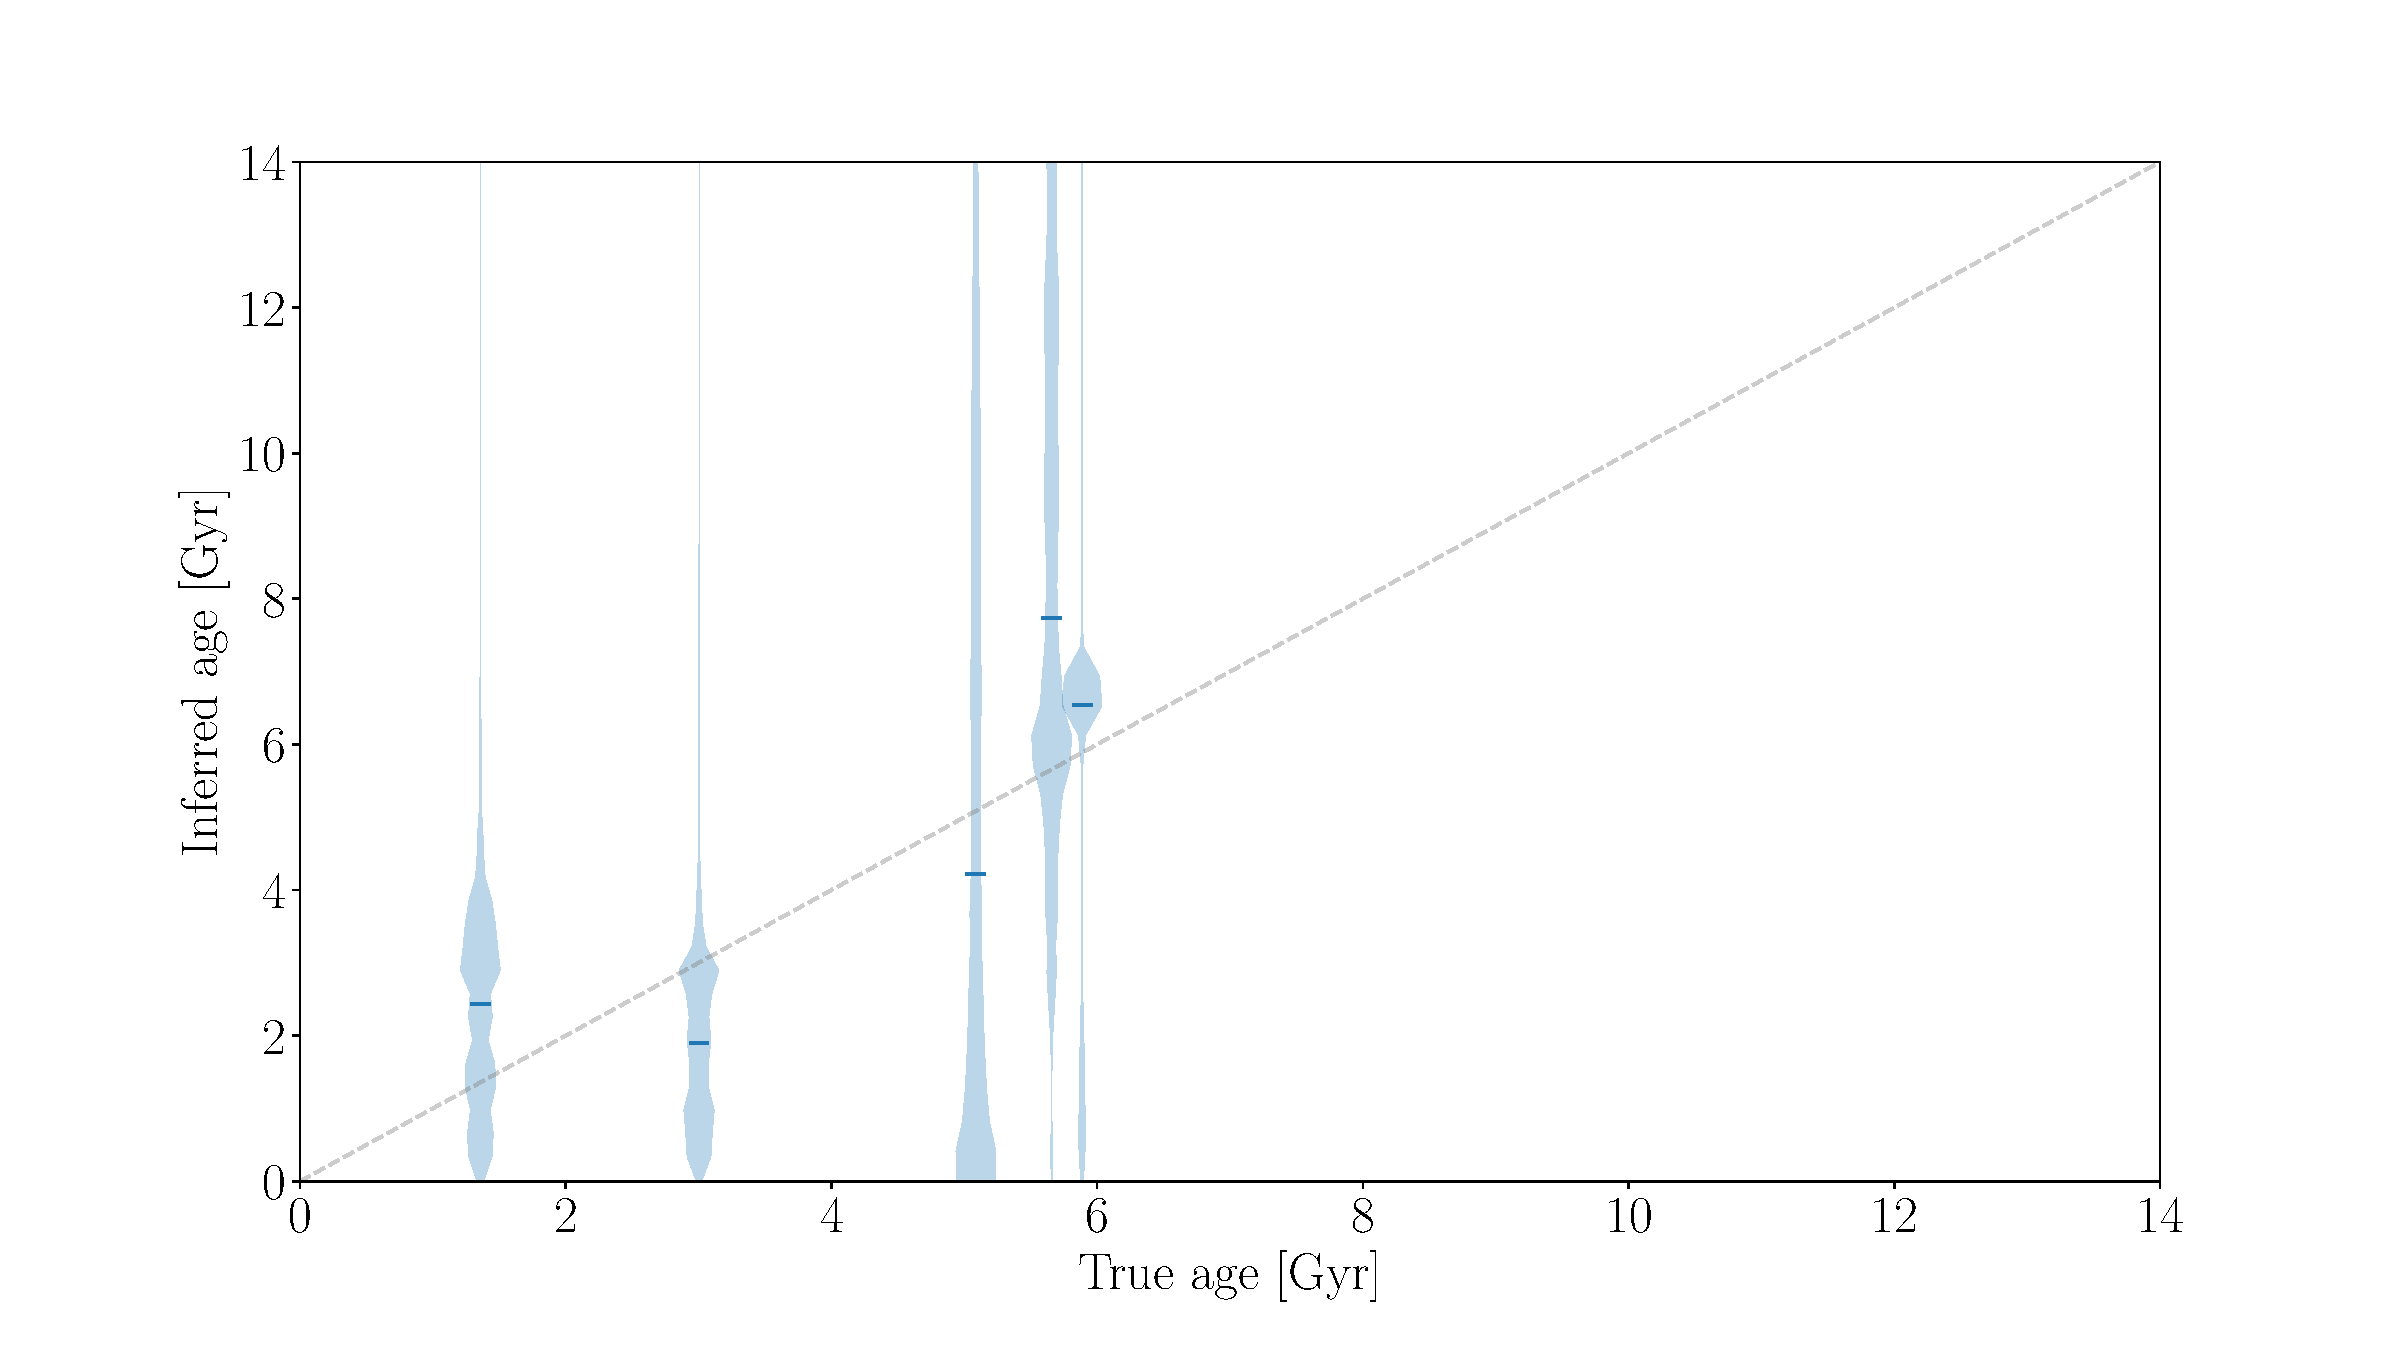
\includegraphics[width=1.1\textwidth]{../plots/iso_only_violin.pdf}
\label{fig:iso_only}
\end{figure}

\begin{figure}
  \caption{
The results of a test in which we simulated observable properties of stars
    with the same model we used to infer their properties.
    In this experiment we used {\it both} stellar evolution models to {\and}
    rotation periods to infer ages.
For results where we used stellar evolution models {\it only}, see the
    previous figure (figure \ref{fig:iso_only}).
The true age, used to produce associated observables is shown on the x-axis,
    and the ages we inferred are shown on the y-axis.
This figure shows the posterior PDFs over stellar age for each of the
    simulated stars as a `violin plot', where samples from the posterior are
    plotted vertically as a smooth, symmetric function.
The widths of these functions indicates the probability over age: wider
    regions represent more probable ages.
The median values of the posterior PDFs are plotted as solid horizontal lines.
    This figure demonstrates that when rotation periods (gyrochronoloy) {\it
    and} stellar evolution models are used to infer the ages of field MS
    stars, the resulting predicted ages relatively precise; much more precise
    than when using stellar evolution models alone.
}
  \centering
    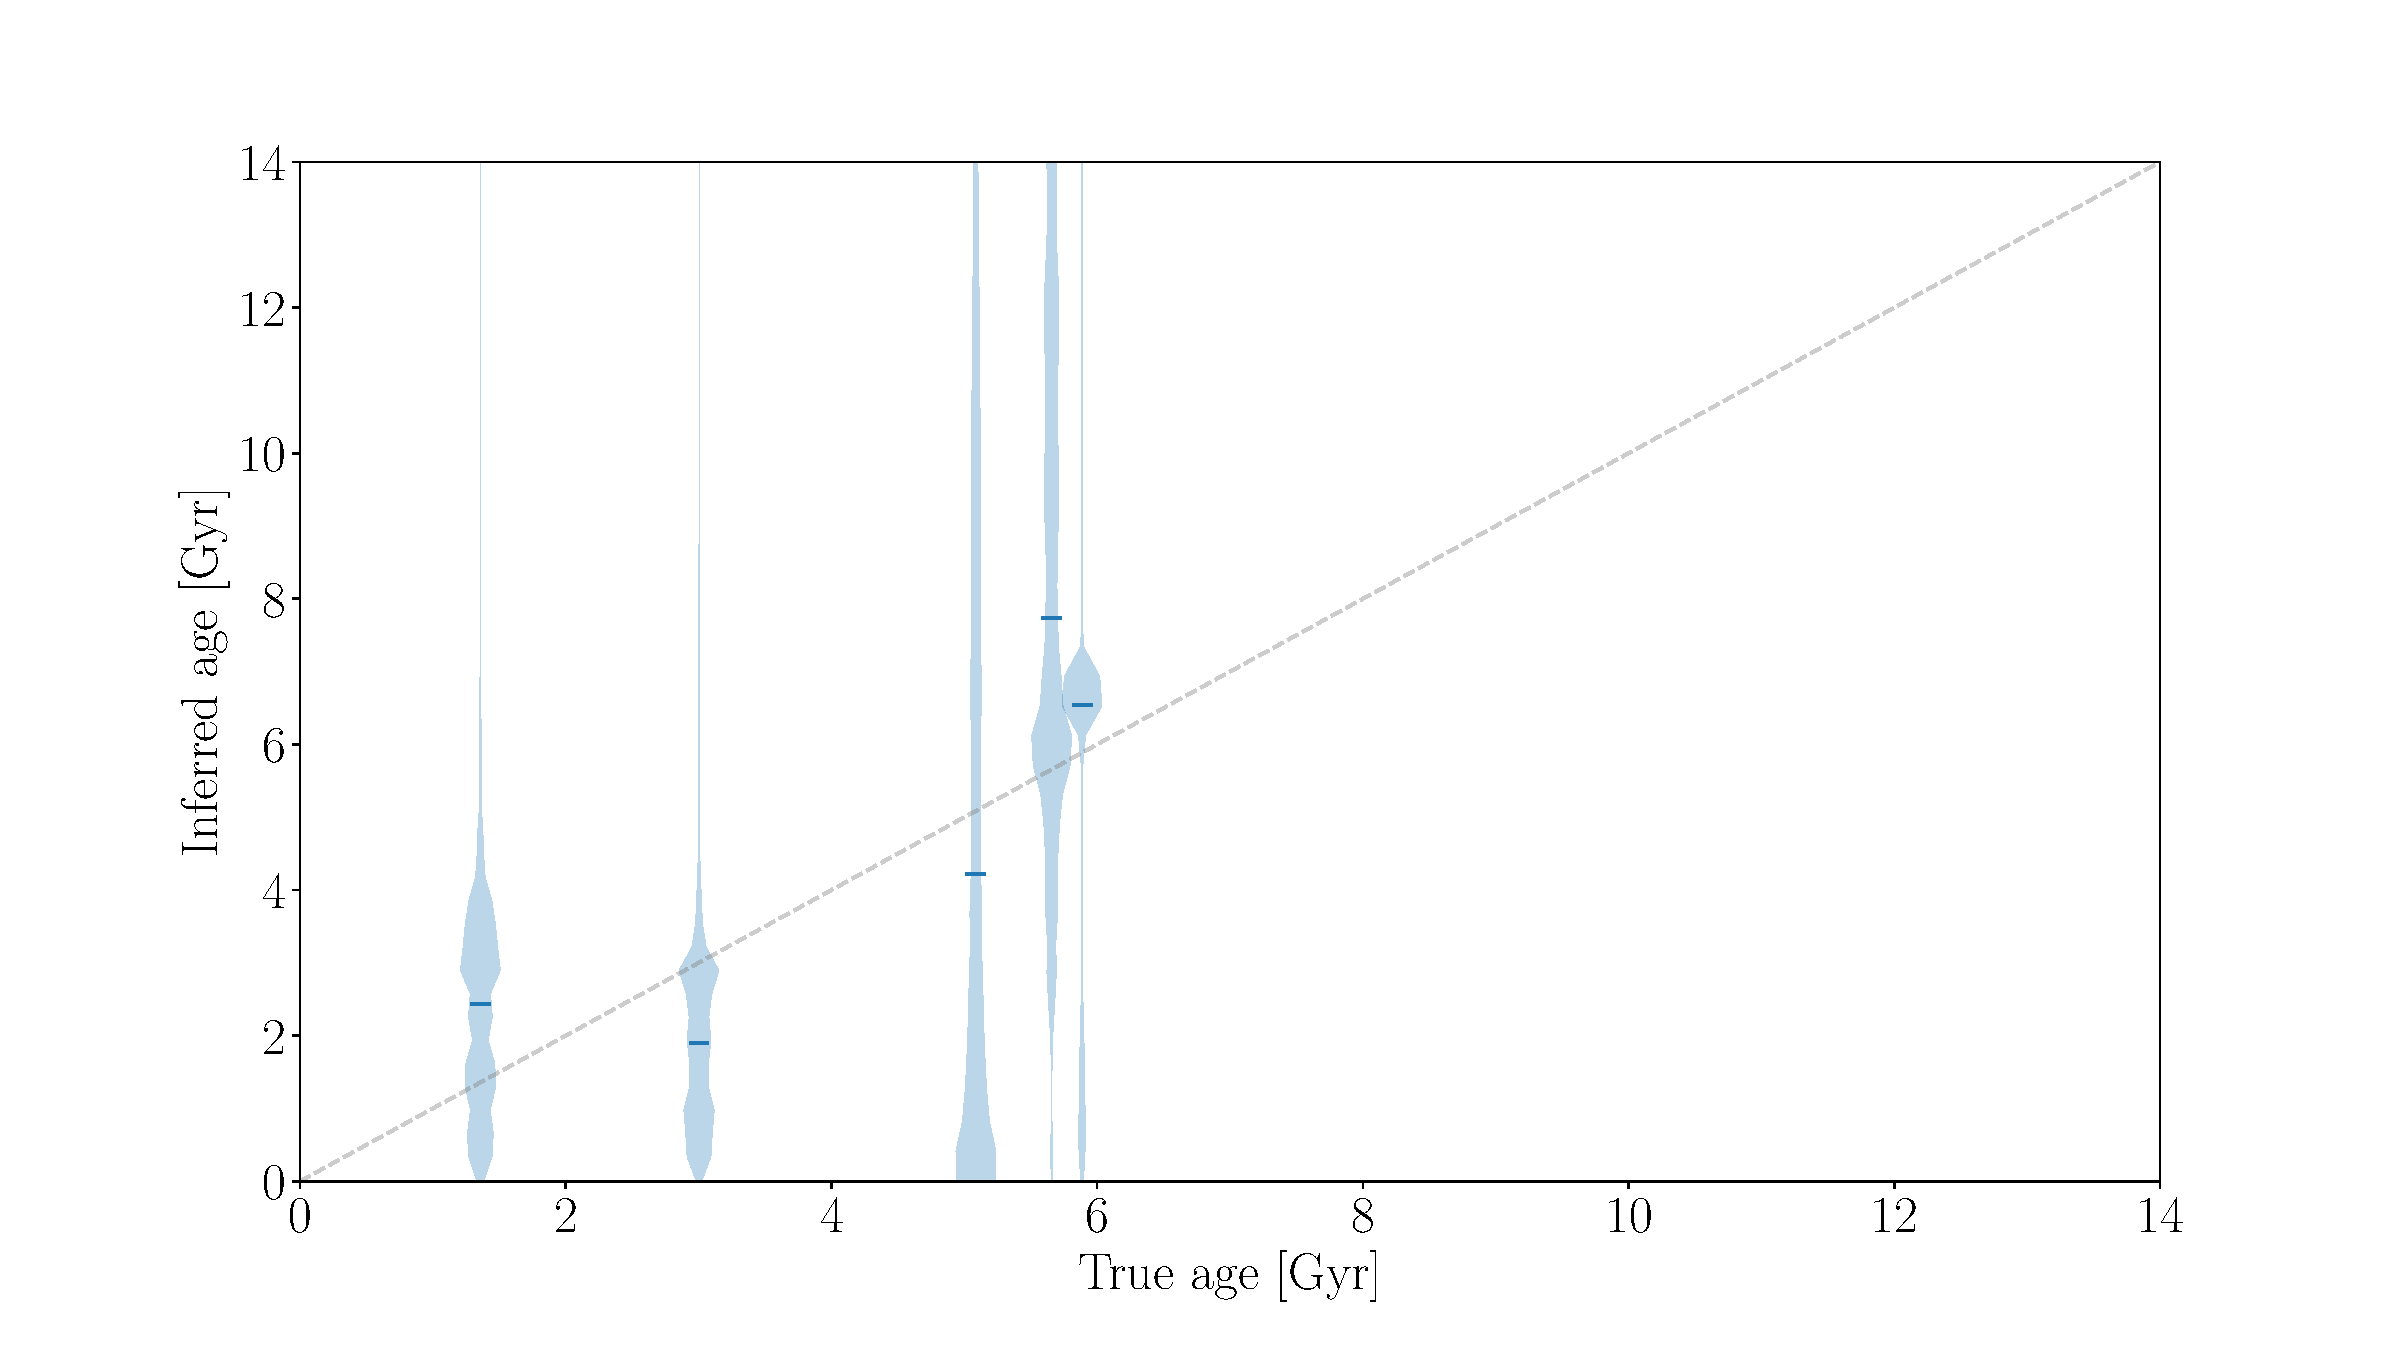
\includegraphics[width=1.1\textwidth]{../plots/iso_only_violin.pdf}
\label{fig:iso_and_gyro}
\end{figure}

%   - The results
Figure \ref{fig:iso_only} shows the results of using a
stellar evolution model model to estimate the posterior PDFs over the stellar
ages of simulated stars.
The rotation periods of stars have not been incorporated into this model:
these posterior PDFs were obtained by isochrone fitting only, using the
likelihood function in equation \ref{eqn:iso_likelihood}.
In most cases ages are only weakly constrained by the stellar evolution
models.
In some cases there is no constraint on the stellar age: the age of the star
is consistent with all ages from 0-14 Gyrs.
The reason for this is that the temperatures and luminosities of stars do not
change very much on the main sequence.
The isochrones are tightly spaced in the MS region of the HR-diagram and, as a
result, even precisely measured temperatures and luminosities often do not
yield precise ages.
Figure \ref{fig:iso_and_gyro} shows the results of using a stellar evolution,
combined with a gyrochronology model.
These ages have been inferred using the likelihood of equation
\ref{eqn:both_likelihood}.
Again, the true stellar ages are plotted on the $x$-axis and the posterior
PDFs of the inferred ages are plotted on the $y$-axis.
Here, unlike the case where only stellar evolution models were used, the
recovered ages are precise.
This is because gyrochronology isochrones (or gyrochrones) are more widely
separated relative to the observational uncertainties than the isochrones used
above.
Put another way, the rotation periods of two stars of different ages and the
same mass will have rotation periods that differ significantly -- almost
certainly more than the observational uncertainty on rotation period.
On the other hand, two stars of the same mass and different age are likely to
have extremely similar luminosities and temperatures and the differences
between these properties are likely to be smaller than the observational
uncertainties.

% We're cheating here.
Figure \ref{gyro_only} demonstrates the results of inferring ages using
rotation periods only, and this illustrates why the combination of isochronal
and gyrochronal ages is so precise: almost all this precision comes from
rotation periods.
This simulation experiment is unrealistic for two main reasons: firstly, we
simulated data from the same gyrochronology model we used to infer ages and so
the results will be perfectly accurate by design.
Secondly, we simulated data without any intrinsic scatter built into the
gyrochronology model; it is a deterministic model.
This means that a rotation period and color predicts a corresponding
single-valued age, rather than a probability distribution over ages.
This is unrealistic given observations of open clusters who's members clearly
show excess scatter in their rotation periods, particularly for less massive
stars.
These results look precise and accurate, but this is misleading.
Inaccuracies would arise if the gyrochronology model was incorrect or poorly
calibrated in all parts of parameter space and imprecision would arise if
intrinsic scatter were built into the gyrochronology model.
The result of using a deterministic model, such as the one used in this
experiment, is that the uncertainties on stellar ages will be unrealistically
small.

%   - Summarize and discuss the experiment.
In this experiment, we compared the precision of MS field star ages inferred
with stellar evolution models only, and with stellar evolution models {\it
combined} with gyrochronology models.
We showed that including gyrochronology in the stellar evolution model results
in much more precise age predictions.
We have not yet made any statement about accuracy however; the above
experiment produces accurate ages by construction.
In order to test the potential of this method to produce accurate results, we
test our model on real data in the following section.

% TEST 4: with and without spectroscopy
% Although inferred ages are likely to be more precise if spectroscopic
% parameters are available (\teff, \logg\ and \feh), it is still possible to
% place constraints on stellar ages if only photometric colors are available,
% especially if the star has a precise parallax measurement.
% Figure \ref{fig:just_photometry} demonstrates the decrease in precision when
% only photometric colors (J, H and K), parallaxes and rotation periods are
% used as observables.
% The top panel of figure \ref{fig:just_photometry} shows an isochrones-only
% model and the bottom panel shows the results of using isochrones {\it and}
% gyrochronology.
% When spectroscopic parameters are not available, including age information
% from a stellar rotation period becomes extremely important as it is far more
% age-sensitive than photometric colors.
% The trade-off, however, is that stellar ages will become gyrochronology
% dominated, and it is even more important to use an accurate gyrochronology
% model.

% TEST 2: Clusters
%-----------------------------------------------------------------------------
%   - The cluster data
In order to test our model on real stars with known ages, we selected a sample
of cluster stars with precisely measured ages from ensemble isochrone fitting
and main sequence turn off.
The ages of open clusters can be measured much more precisely than field
stars for two main reasons.
Firstly, the stars have the same age (to within a few million years), so the
age of a cluster can be inferred with an increased precision that is
proportional to the square root of the number stars, relative to a single star
case.
In addition, stars in the same cluster form (we assume) from the same
molecular cloud and therefore have the same metallicity.
Since cluster stars have the same metallicity and age, stars fall on the same
isochrone and the main sequence turn
off can be identified.
We compiled rotation periods and Gaia photometry and parallaxes for members of
Praesepe, a 650 Myr cluster.
We chose Praesepe because it is relatively tightly clustered on the sky and
many of its members were therefore targeted in a single \ktwo\ campaign, from
which it was possible to measure rotation periods via frequency analysis of
member's light curves \citep{douglas2015}.
% We compiled rotation periods and spectroscopic parameters for members of
% the Pleiades which is 150 million years old, Praesepe, a 650 Myr cluster,
% NGC 6811, 1.1 Myrs and NGC 6819, 2.5 Myrs.
% Rotation periods from the Pleiades \citep{rebull2016} and Praesepe
% \citep{douglas2016} were obtained from frequency analysis of \ktwo\ data, and
% rotation periods for NGC 6811 \citep{meibom2013} and 6819 \citep{meibom2015}
% stars were measured from \kepler\ prime light curves.
We crossmatched N Praesepe members with measured rotation periods
\citep{douglas2015}, with the Gaia DR2 catalog \racomment{Gaia DR2 citation},
using a 5'' search radius.
The result was a sample of N stars with rotation periods, parallaxes and
\gaia\ $G$, $G_{BP}$ and $G_{RP}$ -band photometry.
Figure \ref{figure:praesepe} shows the rotation periods of Praesepe members as
a function of their dust-corrected \gaia\ \gcolor\ colors.
We used the {\tt dustmaps} {\tt python} package to calculate dust extinction
along the line of sight to these stars.
The filled blue circles show the FGK stars on the `rotational main sequence'
that were used to calibrate a relation between rotation period and color for
this cluster.
% REDDENNING!!!!!

% Cutting outliers and limiting color range.
In order to fit a period-color relation to these data we restricted the sample
of cluster stars to the color range, 0.56 $<$ \gcolor\ $<$ 3 in order to
remove early F and late M dwarfs whos' rotation periods do not fall on the
`gyrochronology main sequence'.
Although it {\it may} be possible to crudely predict the ages of these stars
(at least the M dwarfs) from their rotation periods, the age-rotation-color
relation for these stars is very different to the FGK star relations and is
not the focus of this paper.
In addition, we removed rapidly rotating stars from the sample since, although
modeling outliers is important and consequential for gyrochronology in
general, the goal of this paper is not to produce a perfect gyrochronology
that reproduces stochasticity in the data, just a simple function that fits
the rotational main sequence of Praesepe.
In future we plan to update the gyrochronology models to include M dwarfs,
and the outlying rapid rotators using a mixture of Gaussians.
Similarly, we used only Praesepe in this study because the period-color
relations of each open cluster with rotation periods has a different shape.
This is likely due to differences in metalicities, incomplete or noisy
membership lists and differences in rotation period measurement algorithms.
A global gyrochronology calibration, using all cluster data is planned for the
future but, again, is beyond the scope of the project presented here.
The rotation periods of the Praesepe members in the restricted color range and
with outliers removed are plotted against their \Gaia\ colors in figure
\ref{fig:Praesepe}.
We used linear least squares to fit a linear model to Praesepe and the Sun.
A 4th order polynomial in $\log(G_{BP} - G_{RP})$ and a straight line in
$\log(\mathrm{Age~[yrs]})$ was fit to reproduce
$\log(\mathrm{rotation~period~[days]})$.
\begin{equation}
    \log(P) = a + b\log(C_G) + c\log^2(C_G) + d\log^3(C_G) + e\log^4(C_G) +
    f\log(A),
\end{equation}
\label{eq:new_gyro}
were $P$ is period, $C_G$ is \Gaia \gcolor\ color, and A is age.

% Out of a total of N Hyades stars with rotation periods \citep{radick1987,
% radick1995, hartman2011, delorme2011, douglas2016}, N of them have precise
% spectroscopic parameters \citet{brewer}.
% The rest have Gaia photometry ($G$, $G_BP$ and $G_RP$ bands), Kepler
% photometry ($Kp$) and Gaia parallaxes.
% We only selected stars with Gaia DR2 radial velocity (RV) measurements, and
% required that their RVs had to be consistent with the cluster RV of around 40
% kms$^{-1}$.
% Two stars with RVs $< 30$ kms$^{-1}$ were removed from the catalog.

% The Cluster figure
\begin{figure}
  \caption{
% The rotation periods of stars in open clusters, and the Sun, plotted against
%     their \Gaia\ colors (\gcolor) in logarithmic space.
% The result of this fit is plotted on top of the data at the ages of
%     the cluster stars and the Sun.
    The rotation periods of Praesepe members and the Sun, plotted against
    their \Gaia\ colors (\gcolor) in logarithmic space.
    We fit a 4th order polynomial to these data in order to predict
    rotation periods from \gaia\ colors, and a 1st order polynomial (a
    straight line) in age.
The result of this fit is plotted on top of the data at the ages of
    Praesepe and the Sun.
}
  \centering
    \includegraphics[width=1.1\textwidth]{clusters.pdf}
\label{fig:clusters}
\end{figure}

The age of each Praesepe member was inferred using both gyrochronology models:
the legacy model of equation \ref{eq:gyro} and the Praesepe model of equation
\ref{eq:new_gyro}.
This exercise is not designed to test one gyrochronology model against
another: the model fit to the Praesepe data will provide a better age
prediction by design, as the legacy model was fit to number of clusters at
once.
The point of this exercise is to show how precise gyrochronology could be if
the perfect model is used.
We did not force the cluster members to have the same age since the aim of
this experiment was to reveal the precision and accuracy of our method by
quantifying the level of scatter in our predicted ages and identifying regions
of parameter space where the ages deviate from the established age for
Praesepe.

%   - The results
The results are shown in figure \ref{fig:cluster_results} which follows the
same layout as figure \ref{fig:sims_results}.
The top panels shows the ages inferred using an isochrone-only model, the
middle shows a gyrochrone-only model and the bottom shows an isochrone plus
gyrochrone model.
Once again, the top panel demonstrates that using an isochrone model alone
produces imprecise ages.
The middle panel shows ages recovered using only a gyrochronal model and it
reveals inaccuracies in the gyrochronology relation used here.

The bottom panel, once again, demonstrates the power of using both isochronal
and gyrochronal models together to provide a balance of precision and
accuracy.

% TEST 3: Asteroseismology
%-----------------------------------------------------------------------------
%   - The asteroseismic data
%   - The results
